\section{Arquitetura do Sistema}

Para fins de implementação, a arquitetura pode ser organizada em quatro níveis funcionais: sensores, nós de aquisição, gateway e plataforma de dados \cite{5597912,AKYILDIZ2002393}.
Com base nessa organização, os nós realizam a amostragem das variáveis ambientais, associam identificadores e marcas temporais aos dados, executam verificações locais de consistência e encaminham os registros ao gateway \cite{YICK20082292,5597912}.
Por sua vez, o gateway agrega os pacotes recebidos dos nós sensores e os encaminha, por meio de um enlace de backhaul, a um servidor local ou remoto \cite{5597912,10.1145/570738.570751}.
Para preservar a continuidade da aquisição, o armazenamento temporário nos nós ou no gateway permite manter a coleta durante interrupções do enlace de backhaul e transmitir os registros após o restabelecimento da conexão \cite{5597912,10.1145/1031495.1031521}.

A cadeia funcional resultante é apresentada na Figura \ref{fig:arquitetura_funcional}.
Além da organização do fluxo de dados, a implantação exige atenção à autonomia energética, ao encapsulamento, à calibração e à manutenção, pois falhas nesses elementos podem produzir lacunas ou medições sem validade científica \cite{5597912,10.1145/1031495.1031521}.

\begin{figure}[!ht]
    \centering
    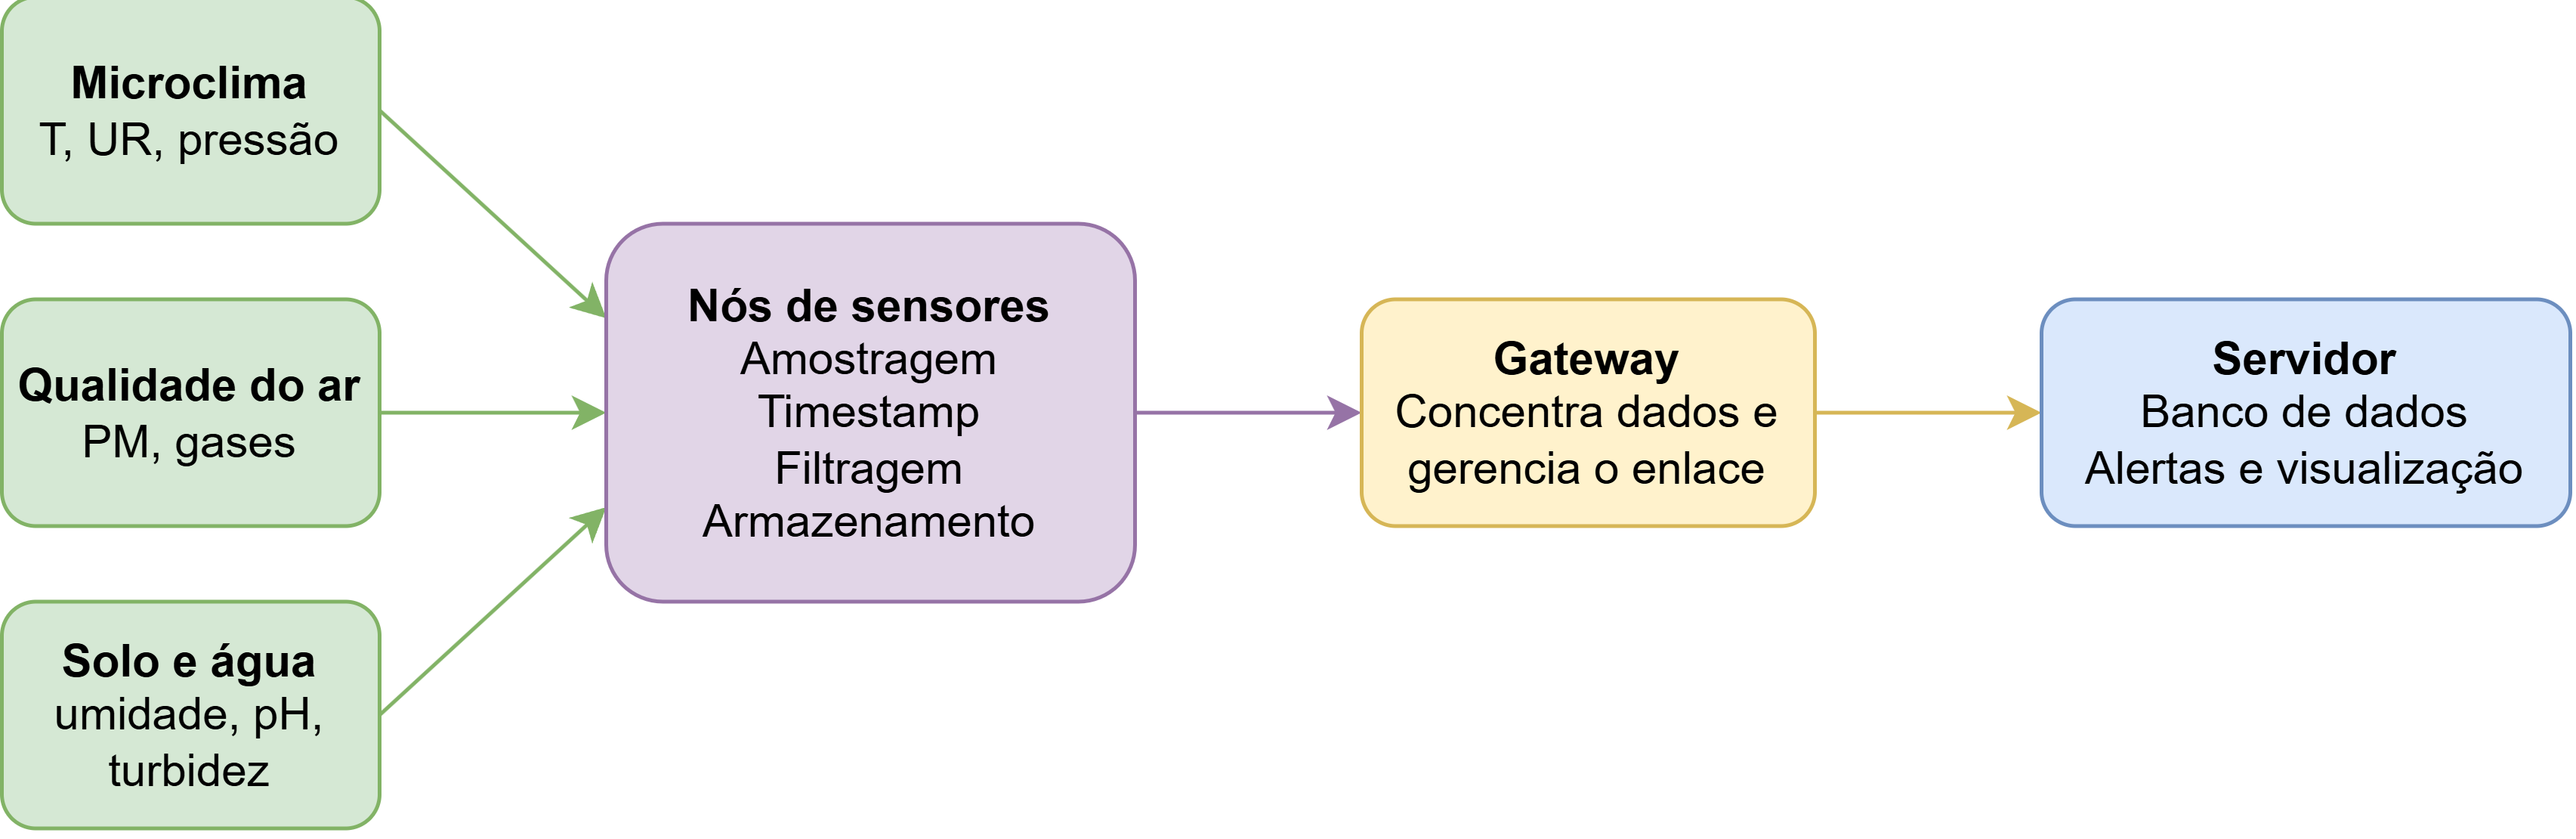
\includegraphics[width=0.98\columnwidth]{figures/arquitetura_funcional.drawio.png}
    \caption{Arquitetura funcional de uma RSSF ambiental.}
    \label{fig:arquitetura_funcional}
\end{figure}